\begin{figure}[ht]
    \begin{subfigure}[t]{0.7\textwidth}
        \caption{}
        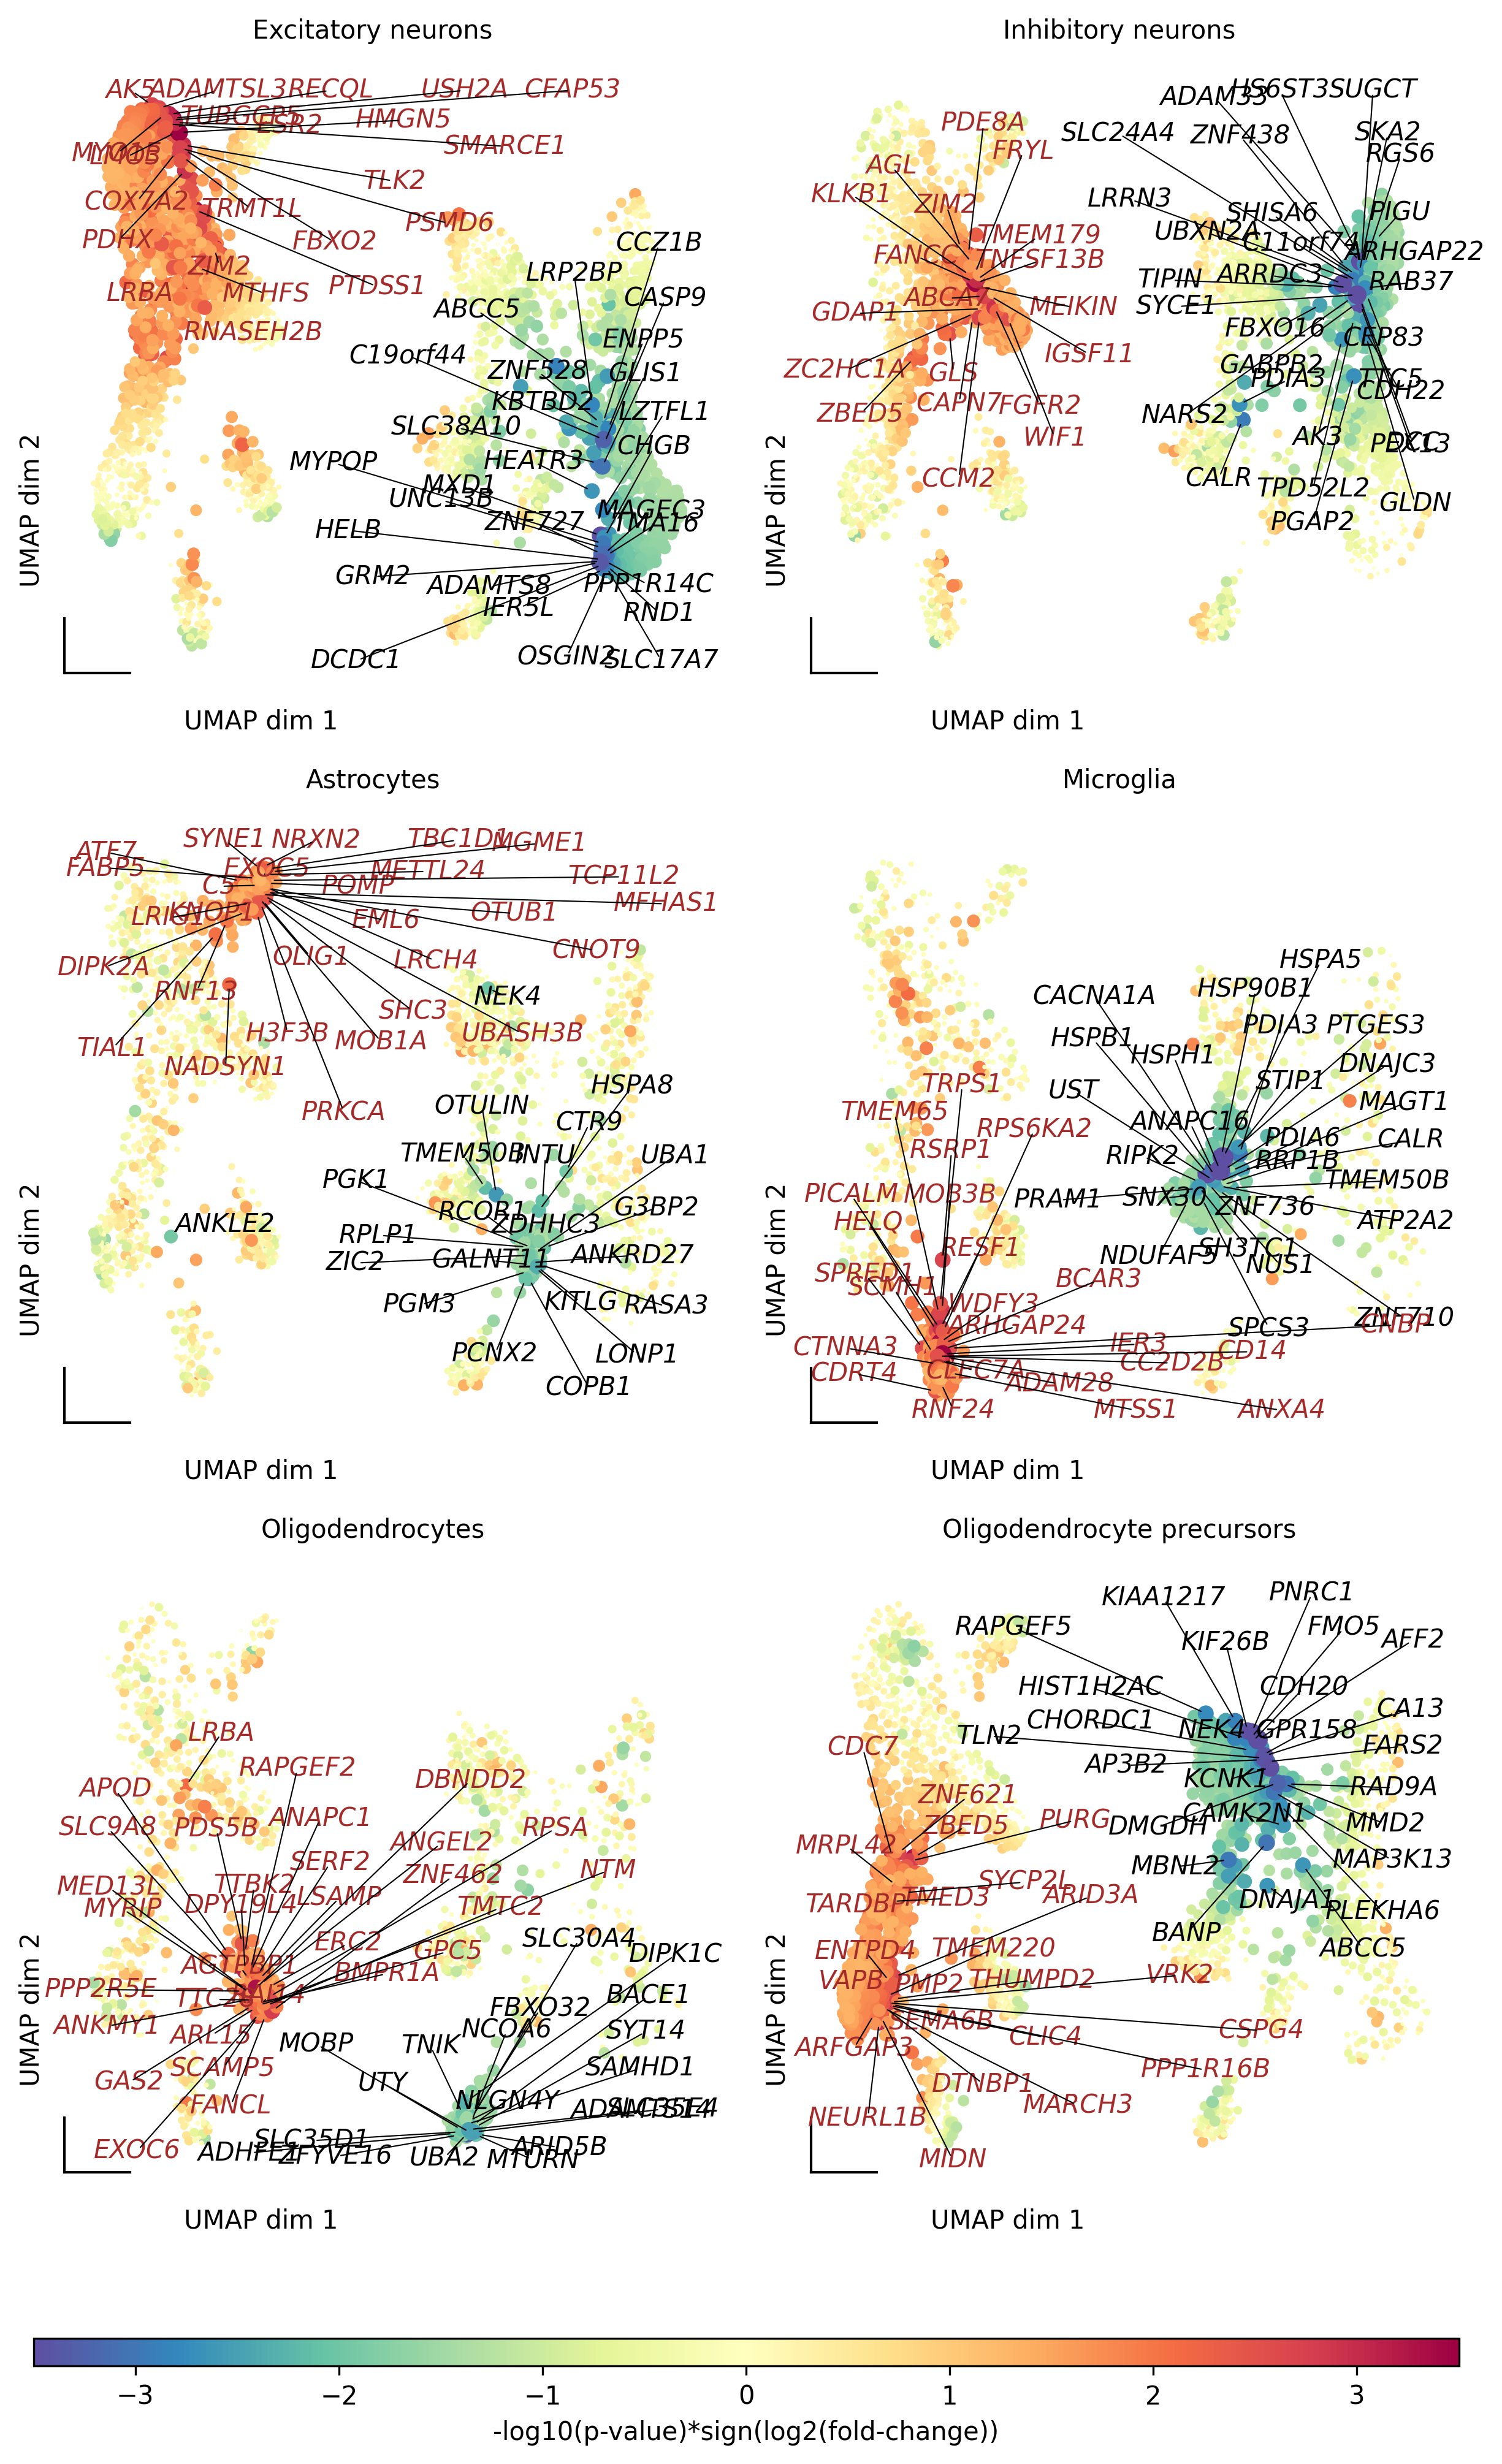
\includegraphics[width=\textwidth]{./extended_plots/umap_projection_more_genes.png}        
    \end{subfigure}    
    \caption{
        \textbf{Single-nuclear RNA-sequencing of Human Post-mortem Prefrontal Cortex Reveals Cell Type-specific Gene Changes in ABCA7 LoF Variant Carriers.}\\[1ex]
        (A) Cartoon overview of gene score analysis strategy (see Methods) (Created with BioRender.com). Genes from cell-type-specific ABCA7 LoF perturbation score space were projected onto the first two UMAP dimensions, followed by clustering and pathway enrichment to provide a unified visual overview of gene expression changes associated with ABCA7 LoF across all major cell types. 
        (B, C) Projections of gene scores onto the top two dimensions computed by UMAP, showing up-regulated genes per cell type ($S > 1.3$) (B) or down-regulated genes per cell type ($S < -1.3$) (C). 
        (D) Perturbation patterns of gene clusters from Figure~\ref{fig:main_atlas}G in indicated cell types shown as histograms (astrocytes (Ast), red; excitatory neurons (Ex), light blue; inhibitory neurons (In), green; microglia (Mic), navy blue; oligodendrocytes (Oli), peach; oligodendrocyte precursor cells (Opc), grey). Gene scores $S$ are plotted on the x-axis and frequency is plotted on the y-axis.
    }
    \label{fig:snRNAseq_gene_scores}
\end{figure}